\section{Security Analysis}
\label{sec:securityAnalysis}

\begin{figure}[t]
\begin{center}
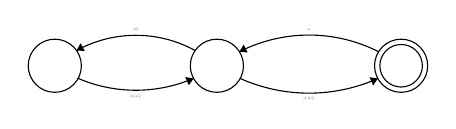
\begin{tikzpicture}[scale=0.15]
\tikzstyle{every node}+=[inner sep=0pt]
\draw [black] (66,-23.1) circle (3);
\draw (66,-23.1) node {\server};
\draw [black] (66,-23.1) circle (2.4);
\draw [black] (45.2,-23.1) circle (3);
\draw (45.2,-23.1) node {\host};
\draw [black] (26.9,-23.1) circle (3);
\draw (26.9,-23.1) node {\user};
\draw [black] (47.743,-21.516) arc (116.95563:63.04437:17.332);
\fill [black] (47.74,-21.52) -- (48.68,-21.6) -- (48.23,-20.71);
\draw (55.6,-19.13) node [above] {$m$};
\draw [black] (29.352,-21.382) arc (118.8302:61.1698:13.89);
\fill [black] (29.35,-21.38) -- (30.29,-21.43) -- (29.81,-20.56);
\draw (36.05,-19.16) node [above] {$[m']$};
\draw [black] (42.565,-24.526) arc (-66.78269:-113.21731:16.527);
\fill [black] (42.57,-24.53) -- (41.63,-24.38) -- (42.03,-25.3);
\draw (36.05,-26.36) node [below] {$(I,[m'])$};
\draw [black] (63.369,-24.535) arc (-65.91058:-114.08942:19.034);
\fill [black] (63.37,-24.53) -- (62.43,-24.4) -- (62.84,-25.32);
\draw (55.6,-26.69) node [below] {$(I,[m'])$};
\end{tikzpicture}
\end{center}
\caption{Finite state machine that depicts the interaction between the user (\user), host (\host) and the server (\server).}
\label{fig:fsm}
\end{figure}

\begin{figure}[t]
\begin{center}
\tikzset{
  % add this style to all tikzpicture environments
  every picture/.append style={
    % enable scaling of nodes
    transform shape,
    % set scale factor
    scale=0.75
  }
  }
\begin{sequencediagram}
\newinst{u}{\user}
\newinst[3]{h}{\host}
\newinst[3]{s}{\server}
\mess{s}{$m$}{h}
\mess{h}{$[m']_1$}{u}
\mess{u}{$I_1,[m']_1$}{h}
\mess{h}{$[m']_2$}{u}
\mess{u}{$I_2,[m']_2$}{h}
\mess{h}{...}{u}
\mess{u}{...}{h}
\mess{h}{$[m']_n$}{u}
\mess{u}{$I_n,[m']_n$}{h}
\mess{h}{$I_1,I_2,...,I_n$}{s}
\mess{h}{$[m']_1,[m']_2,...,[m']_n$}{s}
\end{sequencediagram}
\end{center}
\caption{Protocol transcript between the \server, \user and \host that shows one trace from the FSM depicted in Figure~\ref{fig:fsm}.}
\label{fig:protocol}
\end{figure}


\subsection{Interaction Protocol}

The interaction between the server (\server), user (\user) and host (\host) is depicted in the finite state machine in Figure~\ref{fig:fsm}. \server sends a message $m$ to \host. One can assume $m$ to be the HTML, JS send from \server. We denote $[m]$ to be the render of $m$ by the \host. As \host is malicious, it can transform $m$ to $m'$. Note that the transformation is a public knowledge and is deterministic. If $m\neq m'$ then given $[m]$ and $[m']$, \server can determine that $[m]\neq [m']$. We denote the user input to be $I$ which corresponds to a specific $[m]$. Note that the communication channel between \server to \user is neither authenticated, neither confidential. But the communication channel from \user and \server is authenticated. The user provides both her input $I$ and transformation $[m']$ observed by her to \host. The interaction loop between \host and \user can continue till \user finishes her input. After every input \host hands over new message transformation to \user (either results of the input or new message from \server or both). Once the user provides all her inputs, \host send the pairs $(I, [m'])$ to \server.

We also define two functions:
$$Input():[m]\rightarrow I$$
$$Transform():m,I\rightarrow [m'], \exists i\in I:i=\phi$$
Both of them are \emph{bijective}.

One trace of the protocol transcript is depicted in Figure~\ref{fig:protocol}. As described in the FSM, \server receives traces of message transformation ($[m']_1,[m']_2,\ldots,[m']_n$) and corresponding inputs ($I_1,I_2,\ldots,I_n$). From these traces \server could determine of all the $[m']_i$ are in proper form by verifying if $[m]_i=[m']_i$.

\begin{theorem}
\label{theorem:th1}
If \user does not send all the transformations till $[m']_i$ corresponding to the input $I_i$, input integrity can not be achieved. 
\end{theorem}

\begin{proof}
If \user does not attach all the transformation till $[m']_i$, i.e., $[m']_1, [m']_2, \ldots, [m']_{i-1}, [m']_i$  corresponding to inputs $I_1, I_2,\ldots, I_{i-1}, I_i$, then the server can not verify all the transformations corresponding to the input. \host could modify a specific $[m]_x$ to influence \user input.
\end{proof}

\begin{theorem}
\label{theorem:th2}
If the channel from \user and \server is not authenticated, input integrity is not achievable. But the channel from \server to \user does not require to be secure.
\end{theorem}

\begin{proof}
The proof is trivial. If the channel from \user to \server is not authenticated, any input provided by \user can be manipulated by \host without trace. Hence input integrity is not achievable. As long as \user sends message transformation along with the input, a manipulated message transformation bt \host would be detectable by \server (see Theorem~\ref{theorem:th1}).
\end{proof}


\iffalse
\subsection{Protection against phishing attacks}
\subsection{Keyboard Manipulation Attacks and Defenses}
\subsubsection{Change user selected values}


\subsection{Mouse Manipulation Attacks and Defenses}
\subsubsection{Changing mouse position}
Changing the mouse position can be detected by the device as the device expects to find it in the location that the user provides. 
\subsubsection{Removing the mouse completely}
This is detectable by the \device as the \device no longer finds the mouse pointer in the screen at the designated position.  
\subsubsection{Add mouse cursor to confuse users}

\subsection{UI Manipulation Attacks and Defenses}
\subsubsection{Manipulate the position of the UI elements on the screen}
\fi